\documentclass[a4paper,10pt]{article}
\usepackage[utf8]{inputenc}
\usepackage[T1]{fontenc}
\usepackage{lmodern}
\usepackage[english]{babel}
\usepackage{amsmath, amsfonts, amssymb, amsthm, dsfont}
\usepackage{bbold}
\usepackage{stmaryrd}
\usepackage{mathrsfs}
\usepackage{fancyhdr}
\usepackage{color}
\usepackage{algorithmicx}
\usepackage{graphicx}
\newtheorem{mydef}{Definition}

\begin{document}

\title{MVA Reinforcement Learning\\
Optimization of very difficult functions}

\author{Nathan de Lara, Florian Tilquin}
%\date{}
\maketitle

\section{Introduction}
\subsection{Problem statement}
The goal of this paper is to test and compare recently developed algorithms for the optimization of \textit{very difficult functions}. This work is based on the papers by Bubeck~\cite{bubeck2011x}, Grill~\cite{grill2015black}, Lazaric~\cite{azar2014online}, Bull~\cite{bull2013adaptive} and Valko~\cite{valko2013stochastic}. Each one of this paper has a specific definition of \textit{difficult} but the general idea is that the function to optimize has many local maxima and only one global maximum, it has very fast variations and is not necessarily differentiable such that a gradient-based approach to find the optimum should not be successful. All functions are assumed to be bounded and to have a compact support which, up to scaling can be fixed to be $[0,1]^p$. In this paper, we only consider $p=1$. In the end, the general formulation of the problem is:
\begin{equation}
\mbox{maximize } f(x) \mbox{ for } x\in [0,1]
\end{equation}

\subsection{About the multi-armed bandit}
As previously mentioned, a gradient-based approach is not likely to perform well on the considered functions. Thus, the idea is to use a multi-armed bandit with theoretically an infinite number of arms, sometimes called \textit{continuum-armed bandit}. The algorithms progressively defines a sequence of evaluation points $x_t$ and observes a reward $y_t=f(x_t)+\xi_t$ where $\xi_t$ is a noise term. The choice of $x_{t+1}$ depends on the sequence of $(y_{t'})_{t'\le t}$ and is meant to converge to $x^*$ while controlling the cumulative regret:
\begin{equation}
\label{regret}
R_T = \underset{t=1}{\overset{T}{\sum}}f(x^*)-f(x_t)
\end{equation}
In practice, for the algorithms considered, $x_t = \mathcal{U}(I_t)$. This means that $x_t$ is pulled uniformly at random in an interval $I_t$ that is chosen by the algorithm. The set of intervals defines a tree structure such that the set of leaves is a partition of $[0,1]$. In the end, the original problem is transformed into a particular case of regular multi-armed bandit. Without any prior information on the function to optimize, we only consider here the family of \textit{dyadic trees}. As mentioned in~\cite{bull2013adaptive}, the dyadic tree on [0, 1) is the tree with root node [0, 1), and where each node [a, b) has children $[a, \frac{1}{2}(a+b), [ \frac{1}{2}(a+b), b)$. An example of dyadic tree is displayed in~\ref{dydtree}.

\begin{figure}
\label{dydtree}
\centering
\textbf{A dyadic tree}\\
\end{figure}



\section{Algorithms}
\label{algo}
In this section, we list the algorithms to be compared and briefly present their respective behaviors. The reader is welcome to consult the original papers for more detailed descriptions and proofs on theoretical performances. As previously mentioned, each algorithms defines a sequence of intervals $I_t$ from which $x_t$ is sampled. Typically, the selected interval maximizes a certain selection function of $(x_{t'},y_{t'})_{t'< t}$ among a subset of considered intervals. The main differences in the following algorithms is the definition of the selection function and the choice of the considered intervals at each time step.

\subsection{Hierarchical Optimistic Optimization}

\subsection{Parallel Optimistic Optimization}

\subsection{High-Confidence Tree}

\subsection{Stochastic Simultaneous Optimistic Optimization}

\subsection{Adaptive-Treed Bandits}

\section{Results}
\subsection{Experimental Setup}
\paragraph{Objective functions}
We test the algorithms on different reference functions from~\cite{valko2013stochastic} and~\cite{grill2015black}:
\begin{enumerate}
\item Two-sine product function: $f_1(x) = \frac{1}{2} (\sin(13x) . \sin(27x))+0.5$.
\item Garland function: $f_2(x) = 4x(1-x).(\frac{3}{4}+\frac{1}{4}(1-\sqrt{|\sin(60x)|}))$.
\item Grill function: $f_3(x) = s(\log_2(|x-0.5|).(\sqrt{|x-0.5|}-(x-0.5)^2)-\sqrt{|x-0.5|}$ where $s(x)=\mathbf{1}(x- \lfloor x \rfloor \in [0,0.5])$.
\end{enumerate}
The associated plots are displayed in~\ref{functions}.
\begin{figure}
\label{functions}
\centering
\textbf{Reference functions to optimize}\\
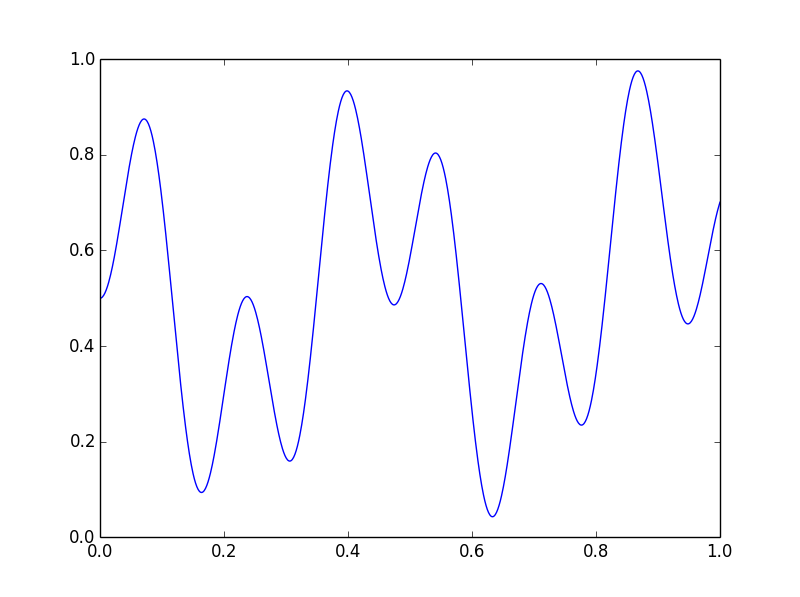
\includegraphics[scale=0.19]{sinprod.png}
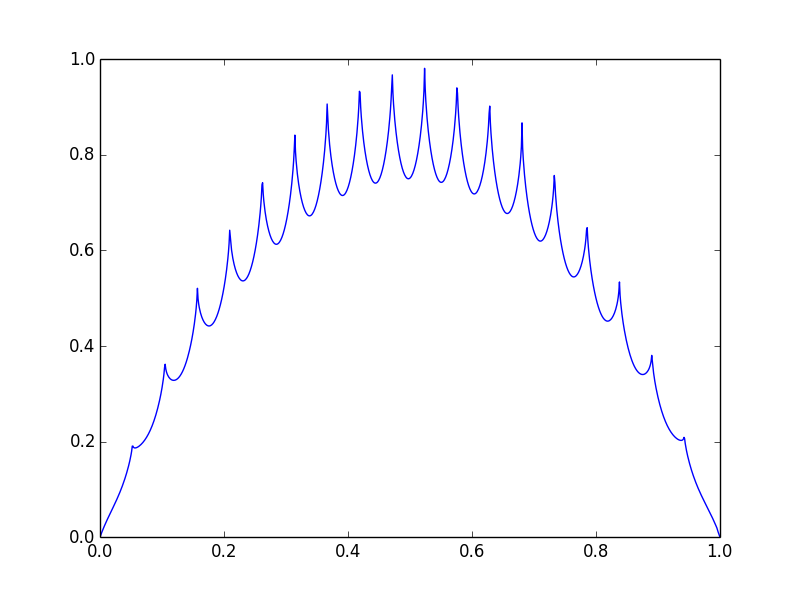
\includegraphics[scale=0.19]{graland.png}
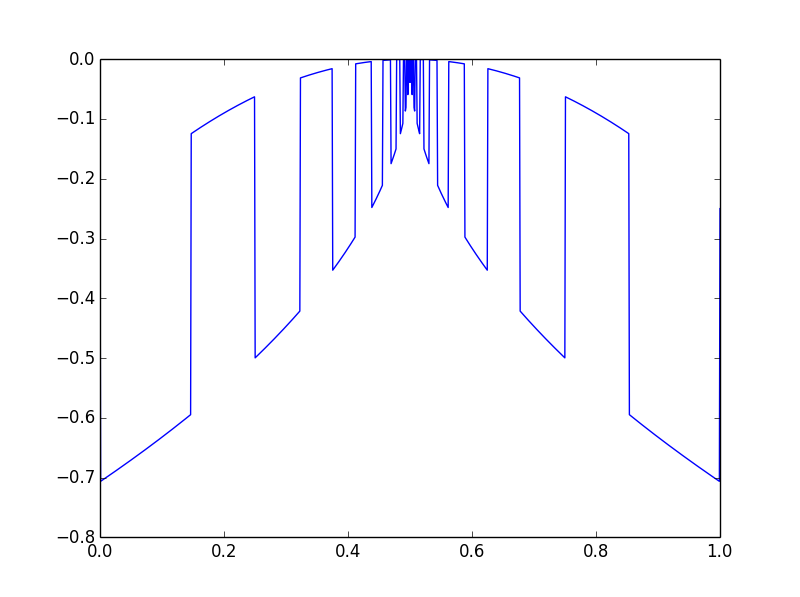
\includegraphics[scale=0.19]{grill.png}
\caption{From the left to the right: Two-sine product, Garlang, Grill.}
\end{figure}

\paragraph{Algorithms setup}
In order to compare the performances of the different algorithms, we set a desired precision $\epsilon$ and a total number of function evaluations $T$ and a number of runs $N$. Then we compute for each and each algorithm run the best value returned $\widehat{x}^*$ and the cumulative regret defined in~\ref{regret}. The run is considered a success if $|\widehat{x}^*-x^*|\le \epsilon$. The success rates are average cumulative regrets are displayed in~\ref{restab}. The tuning of the parameters specific to each algorithm is performed manually.

\begin{figure}
\label{restab}
\centering
\textbf{Success rates and average cumulative regrets of the algorithms}
\begin{tabular}{|l|c|c|c|c|c|c|}
\hline
Algorithm & $f_1$ & $f_2$ & $f_3$ & $\bar{R}_1$ & $\bar{R}_2$ & $\bar{R}_3$ \\
\hline
HOO & & & & & &\\
POO & & & & & &\\
HCT & & & & & &\\
StoSOO & & & & & &\\
ATB & & & & & &\\
\hline
\end{tabular}
\caption{These results are obtained for $\epsilon=$, $T=$ and $N=$.}
\end{figure}

\subsection{Analysis}

\bibliographystyle{plain}
\bibliography{Biblio}{}
\nocite{*}

\label{lastpage}

\end{document}
